\documentclass{beamer}

%% \documentclass[handout]{beamer}
%% % use this with the [handout] option to create handouts for the audience
%% \usepackage{pgfpages}
%% \pgfpagesuselayout{2 on 1}[a4paper,border shrink=5mm]

\mode<presentation>
{
  \usetheme{Diku}
% set this to your preferences:
  \setbeamercovered{invisible}
%  \setbeamercovered{transparent}
}

\usepackage{graphicx}
\usepackage{epic}

\usepackage{amsmath}
\usepackage{amssymb}
\usepackage{amsthm}

\newcommand{\basetop}[1]{\vtop{\vskip-1ex\hbox{#1}}}
\newcommand{\source}[1]{\let\thefootnote\relax\footnotetext{\scriptsize\textcolor{kugray1}{Source: #1}}}

% for coloured code citation in text:
\usepackage{fancyvrb}

%%%%%%%%%%%%%%%%%%%%%%%%%%%%%%%%%
%%%%%    code sections   %%%%%%%%
%%%%%%%%%%%%%%%%%%%%%%%%%%%%%%%%%

% code highlighting commands in own block
\DefineVerbatimEnvironment{code}{Verbatim}{fontsize=\scriptsize}
\DefineVerbatimEnvironment{icode}{Verbatim}{fontsize=\scriptsize}

% Fancy code with color commands:
\DefineVerbatimEnvironment{colorcode}%
        {Verbatim}{fontsize=\scriptsize,commandchars=\\\{\}}

%%%%%%%%%%%%%%%%%%%%%%%%%%%%%%%%%%
%%%%%    some coloring    %%%%%%%%

\definecolor{Red}{RGB}{220,50,10}
\definecolor{Blue}{RGB}{0,51,102}
\definecolor{Yellow}{RGB}{102,51,0}
\definecolor{Orange}{RGB}{178,36,36}
\definecolor{Grey}{RGB}{180,180,180}
\definecolor{Green}{RGB}{20,120,20}
\definecolor{Purple}{RGB}{160,50,100}
\newcommand{\red}[1]{\textcolor{Red}{{#1}}}
\newcommand{\blue}[1]{\textcolor{Blue}{{#1}}}
\newcommand{\yellow}[1]{\textcolor{Yellow}{{#1}}}
\newcommand{\orange}[1]{\textcolor{Orange}{{#1}}}
\newcommand{\grey}[1]{\textcolor{Grey}{{#1}}}
\newcommand{\green}[1]{\textcolor{Green}{{#1}}}
\newcommand{\purple}[1]{\textcolor{Purple}{{#1}}}




% use "DIKU green" from our color theme for \emph
\renewcommand{\emph}[1]{\textcolor{structure}{#1}}
% use some not-too-bright red for an \emp command
\definecolor{DikuRed}{RGB}{130,50,32}
\newcommand{\emp}[1]{\textcolor{DikuRed}{ #1}}
\definecolor{CosGreen}{RGB}{10,100,70}
\newcommand{\emphh}[1]{\textcolor{CosGreen}{ #1}}
\definecolor{CosBlue}{RGB}{55,111,122}
\newcommand{\emphb}[1]{\textcolor{CosBlue}{ #1}}
\definecolor{CosRed}{RGB}{253,1,1}
\newcommand{\empr}[1]{\textcolor{CosRed}{ #1}}

\newcommand{\mymath}[1]{$ #1 $}
\newcommand{\myindx}[1]{_{#1}}
\newcommand{\myindu}[1]{^{#1}}

\newtheorem{mydef}{Definition}
\newtheorem{mytheo}{Theorem}
\newtheorem{mylemma}{Lemma}


%%%%%%%%%%%%%%%%%%%%

\title[Intro]{Introduction:\\Hardware Trends and List Homomorphism}

\author[C.~Oancea]{Cosmin E. Oancea and Troels Henriksen\\{\tt [cosmin.oancea,athas]@diku.dk}}

\institute{Department of Computer Science (DIKU)\\University of Copenhagen}


\date[Sept 2015]{September 2015 PMPH Lecture Notes}


\begin{document}

\titleslide


%%%%%%%%%%%%%%%%%%%%%%%%%%%%%%%%%%%%%%%%%%%%%%%%%%%%%%%%%%%%%%%%%%%%%%
%%%%%%%%%%%%%%%%%%%%%%%%%%%%%%%%%%%%%%%%%%%%%%%%%%%%%%%%%%%%%%%%%%%%%%
%%%%%%%%%%%%%%%%%%%%%%%%%%%%%%%%%%%%%%%%%%%%%%%%%%%%%%%%%%%%%%%%%%%%%%
\begin{frame}[fragile]
	\tableofcontents
\end{frame}

%%%%%%%%%%%%%%%%%%%%%%%%%%%%%%%%%%%%%%%%%%%%%%%%%%%
%%%%%%%%%%%%%%%%%%%%%%%%%%%%%%%%%%%%%%%%%%%%%%%%%%%
%%%%%%%%%%%%%%%%%%%%%%%%%%%%%%%%%%%%%%%%%%%%%%%%%%%

%\section{Scalable Shared Memory Systems}

\section{Introduction$^{\mbox{\bf 2}}$}

\subsection{Brief History}

\begin{frame}[fragile,t]
\frametitle{Introduction$^{\mbox{\bf 2}}$}

\begin{itemize}
    \item Past $>$ 20 years \emph{Information Revolution}:\\
        Explosive growth of semiconductor integration + Internet.\bigskip

    \item Moore's Low 1960s: 
    \begin{itemize}
        \item computing power doubles every 19-24 months 
        \item \emph{system cost effectiveness = {\tt performance/cost} 
                grows exp}.
        \item \alert{CMOS endpoint is near}: miniaturization reaches its limits
                (complementary metal-oxide semiconductor).
    \end  {itemize}\bigskip\pause

    \item Improved Chip Design:
    \begin{itemize}
        \item each new process generation $\Rightarrow$ higher clock rates 
        \item logic switching speed \& amount of on-chip logic increase ($\uparrow$)
        \item better circuit design \& deep pipelines $\Rightarrow$ 
                fewer gate delays / stage
        \item $\uparrow$ on-chip resources $\Rightarrow$ $\uparrow$ throughput by 
                parallelism at all stages. 
    \end  {itemize}\bigskip

    \item Computer Architecture goes back to before 1970s:\\ 
            \emp{How to Best Utilize the ever-increasing ($\uparrow$) Wealth of Resources?}

\end{itemize}

\end{frame}

\begin{frame}[fragile,t]
\frametitle{Brief History}

\begin{itemize}
        \item \emph{ICPP, ISCA 1980/90s: parallel architectures popular topic.}\\
              Demise of SingleCPU System: inevitable \& fast approaching.\bigskip

        \item \alert{Whatever happened? Mid90 Killer-Micro:}
        \begin{itemize}
            \item The rapid increase ($\uparrow$) transistor density $\Rightarrow$\\
            \item path of least resistance: ever-increasing speed of SingleCPU
            \item Complex Out-Of-Order (OoO) processors: 100s instructions/cycle.
            \item Commercial arena: multiprocessors just an uniprocessor extension.
        \end  {itemize}\bigskip

        \item \alert{What Changed?} Multiprocessors Trend: Academia \& Industry:
        \begin{itemize}
            \item \emp{power complexity}
            \item \emp{Memory WALL}: $\uparrow$ performance gap between processor \& memory 
        \end  {itemize}\bigskip

       \item \emph{All Future Architectures adopt some form of massive parallelism!}
\end{itemize}

\end{frame}


\subsection{Computer Architecture Definition}

\begin{frame}[fragile,t]
\frametitle{What used to Be Computer Architecture?}

\begin{columns}\hspace{-8ex}
\column{0.6\textwidth}
\includegraphics[width=44ex]{Figures/L1/SysOrg}
\column{0.65\textwidth}\vspace{-3ex}
\begin{itemize}
    \item Multi-Layered: focus competences.
    \item Each layer uses the ones below it.
    \item \emp{Application} C++/Java/SML/Haskell.
    \item \emp{Compiler}: machine code + OpSys calls.
    \item \emp{OpSys}: extends hardware funct \&
              orchestrates resource sharing among multiple users.
    \item \emp{ISA \& Computer Organization}: 
            software-hardware interface. 
\end{itemize}
\end{columns}

\emp{Old Definition} ISA -- critical role in the success of computer industry:
\begin{itemize}
    \item Early on, used to be the hallmark of system design $\Rightarrow$
    \item Non-Portable Software \& No Compiler at that time
    \item 1960s IBM System360 ISA guarantees backward compatibility $\Rightarrow$
    \item Strategy endured test of time \& Behemoth company today
\end{itemize}
\end{frame}



\begin{frame}[fragile,t]
\frametitle{What Is Computer Architecture Today?}

\begin{columns}
\column{0.59\textwidth}
\hspace{-6ex}\includegraphics[width=44ex]{Figures/L1/SimpleCPU}

\includegraphics[width=39ex]{Figures/L1/SimpleInterconnect}
\column{0.55\textwidth}\vspace{-17ex}
\begin{itemize}
    \item \emp{Much Broader Definition}: how best to build the computer 
            (includes ISA, but focus changed on organization).\medskip

    \item North Bridge: sys bus connects cores to memory \& IO devs.
    \item PCI bus: IO bus connecting North Bridge to high-speed IO 
            to disk, network \& slower dev\medskip

    \item $\leftarrow$ Generic Multiprocessor with Distributed Memory\medskip

    \item \alert{Parallel Sys Main Components:
                (1) Processor, (2) Memory Hierarchy and 
                (3) Interconnection}
\end{itemize}
\end{columns}

\end{frame}



\begin{frame}[fragile,t]
\frametitle{Software-Hardware Synergy \& Biggest Challenge}
\medskip
\begin{columns}
\column{0.33\textwidth}
\includegraphics[width=29ex]{Figures/L1/Synergy}
\column{0.63\textwidth}\vspace{-3ex}
\begin{itemize}
    \item Computer Architect Role:
    \item \emp{design trade-offs across HW/SW interf to meet functional 
            \& performance requirements within cost constraints.}
\end{itemize}
\end{columns}
\medskip

\begin{itemize}
    \item software: flexible approach to simplifying hardware, 
            e.g., TLB exceptions, FP ops,
    \item hardware faster $\Rightarrow$ world of tradeoff in between 
    \item guided by the common case $\Rightarrow$ trends are important.\bigskip

    \item \emp{Important Juncture:} 
        \begin{itemize}
            \item \emph{Higher performance requires Parallel Hardware}
            \item \alert{Biggest Challenge: 
                    develop efficient Massively-Parallel Software!}
        \end  {itemize}
\end{itemize}
\end{frame}

%%%%%%%%%%%%%%%%%%%%%%%%%%%%%%%%%%%%%%%%%%%%%
%%% Please update this when you know how! %%%
%%%%%%%%%%%%%%%%%%%%%%%%%%%%%%%%%%%%%%%%%%%%%
\subsection{Course Organization}
\begin{frame}
\frametitle{Course Organization}

\begin{tabular}{lccccc}
W  & HARDWARE  & & SOFTWARE     & & LAB/CUDA \\\hline\hline
1 & \alert{Trends}         &                         & \emp{List HOM}     & & \emph{Intro \& Simple}\\
  & \alert{Vector Machine} & \emph{$\longleftarrow$} & \emp{(Map-Reduce)} & & \emph{Map Programming}\\\hline
%
2 & In Order & $\longrightarrow$ & VLIW Instr   & & Scan \&\\
  & Processor& $\longleftarrow$ & Scheduling   & & Reduce \\\hline
%
3 & Cache     & & Reasoning About     & & Sparse Vect\\
  & Coherence & & Parallelism   & & Matrix Mult\\\hline
%
4 & Interconnection & & Case Studies \&   & & Transpose \& Matrix\\
  & Networks        & & Optimizations   & & Matrix Mult\\\hline
%
5 & Memory      & & Optimising   & & Sorting \& Profiling \& \\
  & Consistency & & Locality     & & Mem Optimizations \\\hline
%
6 & OoO, Spec   & & Thread-Level   & & Project \\
  & Processor   & & Speculation    & & Work    \\\hline

%\framebox{Processor}       & & \framebox{Low-Level\\Optimizations}        & & \framebox{CUDA: Scan\\Reduce}\\
%$\downarrow$ && $\uparrow$ \\
%\framebox{\red Intermediate code generation} &$\longrightarrow$ & Intermediate code
\end{tabular}
\medskip
%\alert{Keywords: Reasoning, Tradeoffs, Common Case, }

Three narative threads: the path to complex \& good design: 
\begin{itemize}
    \item \emp{Design Space} tradeoffs, constraints, common case, trends.
    \item \emp{Reasoning}: from simple to complex, \emp{Applying Concepts}.
\end  {itemize}
\end{frame}



%%%%%%%%%%%%%%%%%%%%%%%%%%%%%%%%%%%%%%%%%%%%%

\section{Trends of Critical Components of a Parallel System}

\begin{frame}[fragile]
	\tableofcontents[currentsection]
\end{frame}

\subsection{Processor}

\begin{frame}[fragile,t]
\frametitle{Abstractions}
\medskip

\begin{itemize}
%    \item[Program] set of statements performing computational steps.
%    \item[Process/Thread] embeds the execution of the computation.
    \item A \emp{program} is to a \emp{process/thread} 
            what a recipe is for cooking.\smallskip

    \item \emp{Processor (core)}: hardware entity capable of
            sequencing \& executing thread's instructions.\smallskip

    \item \emp{MT Cores} multiple threads, each 
            running in its thread context.\smallskip

    \item \emp{Multiprocessor:} set of processors connected to execute a workload
        \begin{itemize}
            \item mass produced, off-the-shelf, each several cores \& levels of cache
            \item trend towards migrating system functions on the chip:\\
                    memory controllers, external cache directories, network interface
        \end  {itemize}
\end{itemize}

%\begin{columns}
%\column{0.33\textwidth}
%\includegraphics[width=29ex]{Ch1Figs/Synergy}
%\column{0.63\textwidth}\vspace{-3ex}
%\begin{itemize}
%    \item Computer Architect Role:
%    \item \emp{design trade-offs across HW/SW interf to meet functional 
%            \& performance requirements within cost constraints.}
%\end{itemize}
%\end{columns}

\end{frame}


\begin{frame}[fragile,t]
\frametitle{Processor: Clock Frequency/Rate}

Historically the clock rate (at which instr are executed) has increased 
exponentially (1990-2004).

\begin{columns}
\column{0.65\textwidth}
\hspace{-5ex}\includegraphics[width=52ex]{Figures/L1/FreqGraph}\pause
\column{0.48\textwidth}\vspace{-3ex}
\begin{scriptsize}
        \begin{itemize}
            \item $1.19\times$ per-year due technology scaling
                    (same hwd on new techn).

            \item 1990-2002: doubled every $21$ months
                    \alert{Curve $1.49\times$: $30$GHz in 2008!}
            
            \item $1.49\times - 1.19\times$: very-deep (10-20 stages) pipelines!
                    ILP via speculative OoO: register renaming, 
                        reorder buffs, branch prediction, 
                        lockup-free caches, memory disambiguation, etc. 

            \item 2004: Intel cancels Pentium4 @4Ghz \&
                    \emph{Switched Track to Multi-Cores} $\Rightarrow$\\
                    \alert{Tectonic Shift away from muscled deeply-pipelined 
                    uniprocessor.}

            \item \emp{Peaked in 2005, but mostly stalled since 2002!}
                     
        \end  {itemize}
\end{scriptsize}
\end{columns}

\end{frame}


\begin{frame}[fragile,t]
\frametitle{Closer Look at Clock Rate}

\begin{columns}
\column{0.5\textwidth}
\includegraphics[width=40ex]{Figures/L1/FreqGraph}
\column{0.57\textwidth}
        \begin{itemize}
            \item \emph{Technology} (process shrinkage): every generation 
                    transistors' \emph{switching speed increases $41\%$}.\medskip

%                    \item Impact blunted in the future due to \emp{wire delays}
%                                (do not scale)
%                            because speed of wire transmission grows much slower than
%                            switching speed.
%                \end  {itemize}\medskip
            \item \emph{Pipeline Depth:} more stages $\Rightarrow$
                            less complex $\Rightarrow$ less gates/stage
                \begin{itemize}
                    \item \# of gates delays dropped by $25\%$ every process generation.
                \end  {itemize}\medskip

                \item \emph{Improved Circuit Design} 
        \end  {itemize}\bigskip
\end{columns}
\pause

Clock Rate Increase is Not Sustainable:
\begin{itemize}
    \item \emp{Deeper pipelines}: difficult to build useful stages with $<$ 10 gates
    \item \emp{Wire delays:} wire-transm speed $\uparrow$ much 
            slower than switching,
    \item Circuits clocked at \emp{higher rates consume more power}!  
\end  {itemize}

\end{frame}

\begin{frame}[fragile,t]
\frametitle{Processor: Feature Size \& Number of Transistors}

\begin{columns}
\column{0.65\textwidth}
\includegraphics[width=47ex]{Figures/L1/FeatureSize}
\column{0.4\textwidth}
%\begin{scriptsize}
        \begin{itemize}
            \item new process generation every 2 years\smallskip
                
            \item feature size reduced $30\%$ every generation

            \item \# of transistors doubles every 2 years (Moore's low).\\
                    1 Billion in 2008. 
        \end  {itemize}
%\end{scriptsize}
\end{columns}
\vspace{-2ex}

Each process generation offers new resources.
\emp{How best to use the $>100$ billion transistors? Large-Scale CMPs (100s-1000s cores)}:
\begin{itemize}
    \item more cache, better memory-system design
    \item fetch and decode multiple instr per clock
    \item running multiple threads per core and on multiple cores
\end  {itemize} 

\end{frame}

\subsection{Memory}

\begin{frame}[fragile,t]
\frametitle{Memory Systems}

\begin{itemize}
    \item \emp{(Main) Memory Wall:} growing gap between processor and memory speed.
            Processor cannot execute faster than memory system can deliver data 
            and instructions!\bigskip

    \item Want Big, Fast \& Cheap Memory System\smallskip
    \begin{itemize}
        \item access time 
                increases with memory size as it is dominated by 
                wire delays$\Rightarrow$ this will not change in future technologies\smallskip
%(address decoding, address line propagation, bit-line propagation) 
        \item multi-level hierarchies (relies on principle of locality)\smallskip
        \item efficient management is KEY, e.g., cache coherence.\smallskip
        \item Cost and Size memories in a basic PC in 2008:
    \end  {itemize} 
\end{itemize}
\bigskip

\begin{tabular}{|l|l|l|l|l|}\hline
Memory & Size  & Marginal Cost & Cost Per MB & Access Time \\\hline
L2 Cache & 1MB & \$20/MB & \$20 & 5nsec \\\hline
Main Memory & 1 GB & \$50/GB & 5c & 200 nsec \\\hline
Disk & 500GB & \$100/500GB & 0.02c & 5 msec \\\hline
\end{tabular}

\end{frame}


\begin{frame}[fragile,t]
\frametitle{Memory Wall? Which Memory Wall??}

\begin{itemize}
            \item \emph{DRAM density increases $4\times$ every 3 years, BUT} \smallskip

            \item \emp{DRAM speed $\uparrow$ only with $7\%$ per year!} 
                    (processor speed by $50\%$) 

            \item \alert{Perception was that Memory Wall will last forever!}

            \item \emph{Memory Wall Stopped Growing around 2002}.
    
            \item Multi/Many-Cores $\Rightarrow$ shifted from Latency 
                    to \emp{Bandwidth WALL}
\end  {itemize}
\vspace{-3ex}

\begin{columns}
\column{0.65\textwidth}
\includegraphics[width=50ex]{Figures/L1/MemWall}
\column{0.3\textwidth}
\begin{scriptsize}
\begin{itemize}
\item {\tt MemoryWall = mem\_cycle/ proc\_cycle} \smallskip
\item[1990] {\tt MemoryWall = 4} (25MHz,150ns)
\item[2002] exponential growth {\tt MemoryWall = 200} 
\item Stalled since then.
\item If trend continues: 1 Terabit Main Memory by 2021.
\end{itemize}
\end{scriptsize}
\end{columns}

\end{frame}


\begin{frame}[fragile,t]
\frametitle{Disk Memory}

\begin{itemize}
            \item \emph{Historically disk performance improved by $40\%$ per year} \smallskip

            \item {\tt DiskTime=AccessTime+TransferTime} ({\scriptsize {\tt AccessTime=Seek+Latency}})

            \item Historically, transfer time have dominated, but

            \item Today: transfer and access time are of the same \alert{msecs} order
    
            \item Future, Access Time will dominate, but proc-disk gap still large
\end  {itemize}

\begin{columns}
\column{0.5\textwidth}
\includegraphics[width=33ex]{Figures/L1/DISK}
\column{0.5\textwidth}
\includegraphics[width=33ex]{Figures/L1/Disk2}
\end{columns}

{\scriptsize Seek Time: head to reach right track, latency: time to reach the first record on track, both depend on rotation speed \& independent on block size}.

\end{frame}

\subsection{Interconnect}
\begin{frame}[fragile,t]
\frametitle{Interconnection Networks}

Present at many layers:
\begin{itemize}
            \item \emp{On-Chip Interconnects:} forward values between pipeline stages, AND between execution units AND connect cores to shared cache banks. \smallskip

            \item \emp{System Interconnects:} connect processors (CMPs) to memory and IO

            \item \emp{I/O Interconnects}, usually bus e.g., PCI, connect various 
                    devices to the System Bus
            \item \emp{Inter-Systems Interconnects:} connect separate systems (chassis or boxes) \& include
                \begin{itemize}
                    \item \emph{SANs:} connect systems at very short distance
                    \item LANs, WANs (not interesting for us).
                \end  {itemize}

            \item Internet: global world-wide interconnect (not interesting for us).
\end  {itemize}

\end{frame}

%%%%%%%%%%%%%%%%%%%%%%%%%%%%%%%%%%%%%%%%%%%%
%%%%%%%%%%%%%%%%%%%%%%%%%%%%%%%%%%%%%%%%%%%%

\section{Technological Challenges/Constraints}

\begin{frame}[fragile]
	\tableofcontents[currentsection]
\end{frame}


\begin{frame}[fragile,t]
\frametitle{Technological Contraints}

\begin{itemize}
    \item In the Past: tradeoff between cost (area) and time (performance).\bigskip

    \item Today: design is challenged by several technological limits\smallskip
        \begin{itemize} 
            \item \alert{Major new contraint is Power}\smallskip
            \item wire delays\smallskip
            \item reliability\smallskip
            \item complexity of design
        \end  {itemize}\bigskip

    \item \emphh{It seems that parallelism addresses well all these constraints.} 
%    \item Architecture can play a significant role to maintain viability
%            of CMOS technology for years to come.\bigskip

\end{itemize}
\end{frame}

\subsection{Power}

\begin{frame}[fragile,t]
\frametitle{Power}

\begin{itemize}
    \item \emp{\tt Total Power = Dynamic + Static (Leakage)}\\
                        $P_{dynamic} = \alpha C V^2 f$ 
                        consumed by a gate when it switches state\\
                        $P_{static}  = V I_{sub} \sim V e^{-k V_T / T}$ 
                        (caches)\medskip

    \item Dynamic power 
            favors parallel processing over higher clock rate
            \begin{itemize}
                \item $P_{dynamic} \sim F^3$ mostly dissipated in processor\pause
                \item increase clock freq $4\times$ $\Rightarrow$ \pause
                        $4\times$ speedup @ $64\times$ dynamic power!
                \item replicate a uniprocessor $4\times$ $\Rightarrow$ 
                        $4\times$ speedup @ $4\times$ power
            \end  {itemize}\medskip

    \item Static Power: dissipated in all circuits,  
                at all time, nomatter of frequency and whether
                it switches or not.
            \begin{itemize}
                \item negligible 15 years ago, but as feature size 
                        decreased so did the threshold voltage $V_T$ 
                        every generation
                \item \alert{Recently overtook dynamic power as major 
                        source of dissipation!}
            \end{itemize}\medskip

    \item \emp{Power/Energy are Critical Problems}\\ 
                e.g., costly \& many battery operated devices.
%            \begin{itemize}
%                \item Power must be dissipated otherwise temperature
%                        goes up \& affects performance, correctness and
%                        may possibly destroy the circuit, short or long term. 
%                \item Energy depends on power and speed. Costly \& 
%                        many devices are battery-operated devices.
%
%            \end  {itemize}
\end  {itemize}


\end{frame}


\subsection{Reliability}

\begin{frame}[fragile,t]
\frametitle{Reliability}

\begin{itemize}
    \item \emp{Transient Failures (Soft Errors):}
        \begin{itemize}
            \item Charge stored in a transistor \emp{\tt Q = C V}
            \item Supply voltage $V$ decreases every generation\\
                    (consequence of features-size shrinking)
            \item As Q decreases, it is easier to flip bits
            \item Corruption Sources: cosmic rays, alpha particles
                    radiating from the packaging material, electrical noise
            \item Device operational but values have been corrupted
            \item DRAM/SRAM error detection and correction capability
        \end  {itemize}\medskip

    \item \emp{Intermittent/Temporary Failures:}
            \begin{itemize}
                \item last longer, should try to continue execution
                \item aging or temporary environmental variation, e.g., temperature
            \end  {itemize}\medskip

    \item \emp{Permanent Failures:} device will never function again,
                must be isolated \& replaced by spare\medskip

    \item \emph{Chip Mutiprocessors: promote better reliability}
            \begin{itemize}
                \item using threads for redundant execution, 
                \item faulty cores can be disabled $\Rightarrow$ 
                        natural failsafe degradation
            \end  {itemize}
\end  {itemize}
\end{frame}

\subsection{Wire Delays}
\begin{frame}[fragile,t]
\frametitle{Wire Delays}

\begin{itemize}
    \item Miniaturization $\Rightarrow$ transistors switch faster,
            but the propagation delay of signals on wire does not 
            scale as well.\medskip

    \item Wire Delay Propagation $\sim R C$. $R \sim L / CS_{area}$.
            Miniaturization $\Rightarrow$ cross-section area keeps shrinking
                each generation, annuls the benefit of length shrinking. \medskip

    \item Wires can be pipelined like logic.\medskip

    \item Deeper pipelines are better because communication
            limited to only few stages.\medskip

    \item \emph{Impact of wire delays also favors multiprocessors,
            since communication traffic is hierarchical:}
            \begin{itemize}
                \item most communication is local 
                \item inter-core communication is occasional
            \end  {itemize}

\end  {itemize}
\end{frame}

\subsection{Design Complexity}
\begin{frame}[fragile,t]
\frametitle{Design Complexity}

\begin{itemize}
    \item Design Verification has become the dominant cost of chip
            development today, major design constraint.\medskip

    \item \emp{Chip density increases much faster than the productivity 
                of verification engineers} (new tools and speed of systems):
            \begin{itemize}
            \item register-transfer language level, i.e., logic is correct 
            \item core level, i.e., correctness of forwarding, memory disambiguation,
            \item multi-core level, e.g., cache coherence, memory consistency.
            \end  {itemize}\medskip

    \item Vast majority of chip resources dedicated to storage
            also due to verification complexity:
            \begin{itemize}
            \item trivial to increase the size of: 
                caches, store buffers, load/store/ fetch queues, reorder buffers,
                    directory for cache coherence, etc.
            \end  {itemize}\medskip

    \item \emph{Design Trend Favors Multiprocessors:}
            easier to replicate the same structure multiple times
            than to design a large, complex one.
\end  {itemize}
\end{frame}

\subsection{CMOS Endpoint}
\begin{frame}[fragile,t]
\frametitle{CMOS (Endpoint) Meets Quantum Physics}

\begin{itemize}
    \item CMOS is rapidly reaching the limits of miniaturization,\medskip

    \item Feature size: half pitch distance (half the distance between
            two metal wires). Gate length $\sim 1/2$ feature size.\medskip

    \item If present trends continues feature size $< 10 nm$ by 2020\medskip

    \item Radius of atom: $0.1 \sim 0.2 nm$ $\Rightarrow$ gate length quickly
            reaches atomic distances that are governed by quantum physics,
            i.e., binary logics replaced with probabilistic states.\medskip

    \item Not clear what will follow (?)
\end  {itemize}
\end{frame}

%%%%%%%%%%%%%%%%%%%%%%%%%%%%%%%%%%%%%%%%%%%%%%%%%%%%%%%%%%%%%%%%%%%%%%
%%%   Metrics (Performance, Speedup, Amdhal and Gustafsson laws)   %%%
%%%%%%%%%%%%%%%%%%%%%%%%%%%%%%%%%%%%%%%%%%%%%%%%%%%%%%%%%%%%%%%%%%%%%%

\section{How to Reason about Parallelism?}

\begin{frame}[fragile]
	\tableofcontents[currentsection]
\end{frame}

\subsection{Amdahl's Law}

\begin{frame}[fragile,t]
\frametitle{Amdahl's Law}
\vspace{-5ex}
\includegraphics[width=47ex]{Figures/L1/Amdhal}
\vspace{-7ex}

Enhancement accelerates a fraction $F$ of the task by a factor $S$:\bigskip

\centering{$T_{exe}(with E) = T_{exe}(without E)\times[(1-F) + \frac{F}{S}]$}\bigskip

\centering{$Speedup(E) = \frac{T_{exe}(without E)}{T_{exe}(with E)} = \frac{1}{(1-F)+\frac{F}{S}}$}

\end{frame}

\begin{frame}[fragile,t]
\frametitle{Amdahl's Law}

\begin{itemize}
    \item[1] Improvement is limited by the $1-F$ part of the execution 
                that cannot be optimized:
                $Speedup(E) < \frac{1}{1-F}$\medskip

    \item[2] Optimize the common case \& execute the rare case in software.

    \item[3] Low of diminishing returns\smallskip

\end{itemize}

\vspace{-4ex}
\begin{columns}
\column{0.7\textwidth}
\includegraphics[width=55ex]{Figures/L1/AmdhalDimRet}\pause
\column{0.5\textwidth}\vspace{-3ex}
\begin{itemize}
    \item every increment of $S$\\ consumes new resources\\
            and is less rewarding: 
    \item $S = 2 \Rightarrow 33\%$ speedup,
    \item $S = 5 \Rightarrow 6.67\%$ speedup.
\end{itemize}
\end{columns}

\end{frame}


\begin{frame}[fragile,t]
\frametitle{Amdahl's Law: Parallel Speedup}

\centering{$S_P = \frac{T_1}{T_P} = \frac{P}{F+P(1-F)} < \frac{1}{1-F}$}\medskip

\begin{columns}
\column{0.6\textwidth}
\includegraphics[width=44ex]{Figures/L1/ParSpeedup}
\column{0.5\textwidth}\vspace{-5ex}
\begin{itemize}
    \item Typically: speedup is sublinear, e.g., due to inter-thread communic. 
    \item Sometimes superlinear speedup due to cache effects.
    \item Unforgiving Law: even if $99\%$ is parallelized, $S_{\infty} < 100$.
\end{itemize}
\end{columns}

\pause
\vspace{-3ex}

Hardware Trend is to ever increase the number of cores.\\
\alert{Amdhal's Law: reason about parallelism asymptotically ($\infty \ \#$ cores),\\
i.e., systematically exploit all levels of application's parallelism.}

\end{frame}


%%%%%%%%%%%%%%%%%%%%%%%%%%%%%%%%%%%%%%%%%%%%%%%%
%%% REMOVED FROM THIS LECTURE THE PART ABOUT %%%
%%%      "VECTOR and ARRAY PROCESSORS"       %%%
%%%%%%%%%%%%%%%%%%%%%%%%%%%%%%%%%%%%%%%%%%%%%%%%


\subsection{List Homomorphism}

\begin{frame}[fragile]
	\tableofcontents[currentsubsection]
\end{frame}

\begin{frame}[fragile,t]
\frametitle{Math Preliminaries: Monoid \& Homomorphism}

\begin{mydef}[Monoid]\label{MonoidDef}\vspace{-1ex}
Assume set $S$ and $\odot : S \times S \rightarrow S$.
\emp{$(S, \odot)$ is called a Monoid} if it satisfies the following two axioms:\\
\emp{(1) Associativity:} $\forall x,y,z\in S$ we have 
    $(x \odot y) \odot z \equiv x \odot (y \odot z)$ and\\
\emp{(2) Identity Element:} $\exists e \in S$ such that $\forall a \in S$, %we have
    $e \odot a \equiv a \odot e \equiv a$.\\\medskip

($(S,\odot)$ is called a group if it also satisfies that any element is 
    invertible, i.e., 
    $\forall a, \exists a^{-1}$ such that 
    $a\odot a^{-1}\equiv a^{-1}\odot a\equiv e$.)
\end{mydef}

E.g., $(\mathbb{N},+)$, $(\mathbb{Z},\times)$, $(\mathbb{L}_T,++)$, where\\
        $\mathbb{L}_T$ denotes lists of elements of type $T$,
        and $++$ list concatenation. 

\pause

\begin{mydef}[Monoid Homomorphism]\label{HomDef}\vspace{-1ex}
\emp{A monoid homomorphism} from monoid $(S,\oplus)$ to monoid $(T,\odot)$
is a function $h : S \rightarrow T$ such that $\forall u, v\in S$,
\emp{$h(u\oplus v) \equiv h(u)\odot h(v)$}.
\end{mydef}

%\alert{This has a shape similar to divide and conquer algorithms!}

\end{frame}


\begin{frame}
  \frametitle{List Homomorphism (LH)}

\begin{itemize}
    \item Finite lists with concatenation, denoted {\tt ++}, forms a Monoid:
        \begin{itemize}
            \item {\tt [1,2,3,4] ++ [5,6,7,8] = [1,2,3,4,5,6,7,8]},
            \item neutral elem $e_{\tt++}$ is the empty list {\tt[]}, 
                i.e., {\tt [1,2]++[] = [1,2]},
            \item later we will look at them as \emph{vectors} rather 
                    than \alert{linked lists}.
        \end{itemize}
%    \item Motivation: a large class of list-homomorphic function have 
%            {\em efficient data-parallel} (map-reduce style) implementations!
\end{itemize}
\pause

\begin{mydef}[List Homomorphism]\label{LHomDef}
$h :: [T_1] \rightarrow T_2$ over finite lists is a {\em list homomorphism}
if there exists a(n associative) binary operator $\odot :: T_2 \rightarrow T_2 \rightarrow T_2$,
such that: \\
$\mbox{ }\mbox{ }\mbox{ }\mbox{ }\mbox{ }\mbox{ }\mbox{ }\mbox{ }\mbox{ }$
\emp{$h \mbox{ } (x{\tt ++}y) = (h\mbox{ }x)\mbox{ }\odot\mbox{ }(h\mbox{ }y)$} \\
We denote $h = hom \mbox{ }(\odot) \mbox{ }f\mbox{ }e$, where $f(x) = h([x])$ 
and $e = h([])$. 
\end{mydef}

\begin{itemize}
    \item If the program is well behaved, i.e., same result
            for any {\tt x++y} splitting of the input list, 
            then $(T_2,\odot)$ is necessarily a Monoid.\smallskip

    \item Similar to a divide and conquer algorithm, where 
            {\tt h(x)} and {\tt h(y)} can be computed in parallel 
            and results can be merged. 
\end{itemize}
\end{frame}


\begin{frame}[fragile,t]
  \frametitle{List Homomorphism (LH) Examples}

%Those functions that promote through list concatenation ({\tt ++}):
%$h\mbox{ }(x {\tt ++} y) = (h\mbox{ }x) \odot (h\mbox{ }y)$. More precise:

\begin{mydef}[List Homomorphism]\label{LHomDef}
$h :: [T_1] \rightarrow T_2$ over finite lists is a {\em list homomorphism}
if there exists an associative binary operator $\odot :: T_2 \rightarrow T_2 \rightarrow T_2$,
such that: \\
$\mbox{ }\mbox{ }\mbox{ }\mbox{ }\mbox{ }\mbox{ }\mbox{ }\mbox{ }\mbox{ }$
\emp{$h \mbox{ } (x{\tt ++}y) = (h\mbox{ }x)\mbox{ }\odot\mbox{ }(h\mbox{ }y)$} \\
We denote $h = hom \mbox{ }(\odot) \mbox{ }f\mbox{ }e$, where $f\mbox{ }x = h\mbox{ }[x]$ and $e = h\mbox{ }[]$. 
\end{mydef}

\begin{block}{Examples of List Homomorphisms, id x = x is the identity function}
\vspace{-2ex}
\begin{columns}
\column{0.45\textwidth}
\begin{colorcode}[fontsize=\scriptsize]
-- \emp{len} = \emp{hom (+) one 0}, one x = 1
len :: [T] -> Integer
len []     = \emp{0}
len [x]    = \emp{1}
\emph{len} (x++y) = (\emph{len} x) \emp{+} (\emph{len} y)

-- \emph{flatten} = \emp{hom (++) id []}
flatten :: [[T]] -> [T]
flatten []     = \emp{[]}
flatten [x]    = \emp{x}
\emph{flatten} (x++y) = (\emph{flatten} x) \emp{++} 
                 (\emph{flatten} y)
\end{colorcode}
\column{0.45\textwidth}
\begin{colorcode}[fontsize=\scriptsize]
-- \emph{maxList} = \emp{hom (max) id \mymath{-\infty}} 
maxList :: [Int] -> Int
maxList []     = \emp{\mymath{-\infty}}
maxList [x]    = \emp{x}
\emph{maxList} (x++y) = (\emph{maxList} x) \emp{`max`} 
                 (\emph{maxList} y)
-- Assume p :: T -> Bool given,
-- \emph{all\mymath{\myindx{p}}} = \emp{hom (&&) p True}
all\mymath{\myindx{p}} :: [T] -> Bool
all\mymath{\myindx{p}} []     = \alert{???}
all\mymath{\myindx{p}} [x]    = \alert{???} 
\emph{all\mymath{\myindx{p}}} (x++y) = \alert{???}
\end{colorcode}
\end{columns}
\end{block}

%\emp{True}
%\emp{p x}
%(\emph{all\mymath{\myindx{p}}} x) \emp{&&} (\emph{all\mymath{\myindx{p}}} y)

%Definition~\ref{LHomDef} implies

\end{frame}


\begin{frame}[fragile,t]
  \frametitle{Exercise: Implement the above LHs in Haskell}

\begin{block}{Implementation Sample for all$_p$:} 
\begin{colorcode}[fontsize=\scriptsize]
import System.Environment -- access to arguments etc.
-- helper to simulate (x++y) pattern
split :: [a] -> ([a], [a])
split []  = ([],[] )
split [x] = ([],[x]) 
split xs  = let mid = (length xs) `div` 2  in  (take mid xs, drop mid xs)

-- \emph{all\mymath{\myindx{p}}} \mymath{\equiv} \emph{alln p} = \emp{hom (&&) p True}
\emph{alln} :: (a -> Bool) -> [a] -> Bool
\emph{alln p} []     = True
\emph{alln p} [x]    = p x
\emph{alln p} xs     = let (x, y) = split xs   in   (\emph{alln p} x) && (\emph{alln p} y)

----- Compile with: ghc -O2 -o test LHegHaskell.hs -----
main :: IO()
main = do args <- getArgs
          let inp = if null args then [0,2,4,6] else read (head args)
              p x = x `mod` 2 == 0
              res = alln p inp  
          putStrLn ("Computed: " ++ show res)
\end{colorcode}
\end{block}
\end{frame}

\subsection{List-Homomorphism $\equiv$ Map-Reduce}
\begin{frame}[fragile]
	\tableofcontents[currentsubsection]
\end{frame}

\begin{frame}[fragile,t]
   \frametitle{Basic Blocks of Parallel Programming: Map}

\bigskip

\emp{map} :: $((\alpha \rightarrow \beta), [\alpha]) \rightarrow [\beta] $ has \emph{\em inherently parallel semantics}.


\bigskip

\begin{tabular}{crcccccl}
x = & \emp{map}(~~~f, \{& $a_1$, & $a_2$, & .., & $a_n$ & \} & )\\
    &      & $\downarrow$ & $\downarrow$ &  & $\downarrow$ & &\\
x $\equiv$ &  \{  & \emph{f($a_1$)}, & \emph{f($a_2$)}, & .., & \emph{f($a_n$)} & \} &
\end{tabular}

\bigskip
\bigskip

\emp{Map Fusion:} (higher-order transformation)

\begin{tabular}{rccc}
a = & \{ $a_1$, $a_2$, .., $a_n$ \} & & a = \{ $a_1$, $a_2$, .., $a_n$ \} \\  
\emp{x =} & \emp{map( f, a )} & & \\
%  & $\downarrow$ & & \\
%//x = &  \{ \emph{f($a_1$)}, \emph{f($a_2$)}, .., \emph{f($a_n$)} \} & & \\
\emph{y} = & \emp{map( g, x )} & $\equiv$ & \emph{y} = \emp{map(g o f, a)}\\
  & $\downarrow$ & & \\
\emph{y} $\equiv$ &  \{\emph{g(f($a_1$))},\emph{g(f($a_2$))},..,\emph{g(f($a_n$))}\} & $\equiv$ & \{\emph{g(f($a_1$))},\emph{g(f($a_2$))},..,\emph{g(f($a_n$))}\} \\
\end{tabular}

\end{frame}


\begin{frame}[fragile,t]
   \frametitle{Basic Blocks of Parallel Programming: Reduce}

\bigskip

\emp{reduce} :: $((\alpha \rightarrow \alpha \rightarrow \alpha), \alpha, [\alpha]) \rightarrow \alpha$

\smallskip

\emp{reduce}($\odot$, $e$, \{$a_1$, $a_2$, ..., $a_n$\}) $\equiv$ \emph{$e \odot a_1 \odot a_2 \odot ... \odot a_n$}

\smallskip

~~~~~where $\odot$ is an associative binary operator.

\bigskip

\begin{center} 
        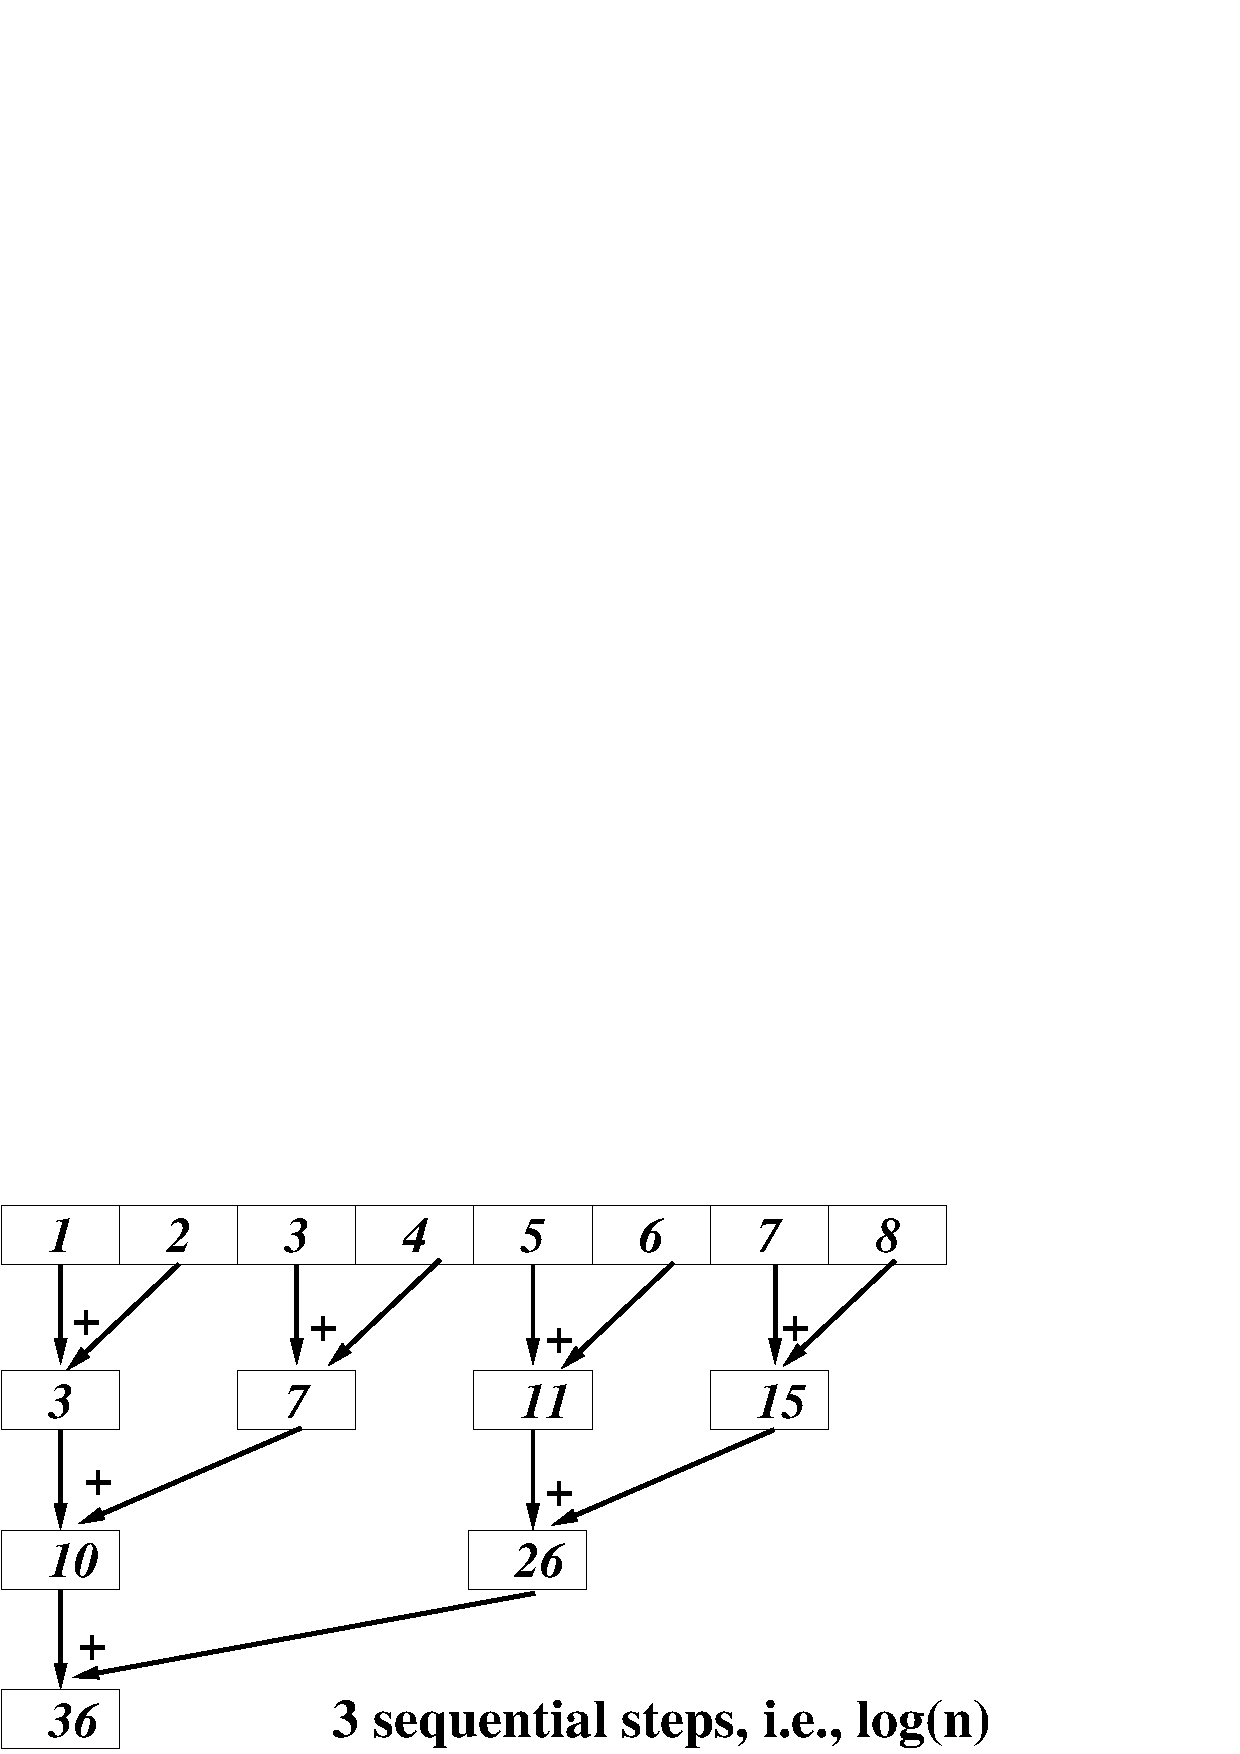
\includegraphics[height=25ex]{Figures/ReduceEg.pdf} 
\end{center} 

Build programs by combining \emp{map}, \emp{reduce} and other such operators. %Example: \smallskip

\end{frame}


\begin{frame}[fragile,t]
  \frametitle{Map, Reduce, and Scan Types and Semantics}

\begin{itemize}
    \item \emp{\tt map~::~($\alpha\rightarrow\beta$)~$\rightarrow$~[$\alpha$]$~\rightarrow$~[$\beta$]}\\
    \emph{\tt map f [x$_1,\ldots, $x$_n$] = [f(x$_1$),$\ldots$, f(x$_n$)]},\\  
        i.e., \emp{\tt{}x$_i$~::~$\alpha, \forall i$}, and 
        \emp{\tt f~::~$\alpha\rightarrow\beta$}.\medskip

    \item \emp{{\tt reduce~::~($\alpha$~$\rightarrow$~$\alpha$~$\rightarrow$~$\alpha$)~$\rightarrow$~$\alpha$~$\rightarrow$~[$\alpha$]~$\rightarrow$~$\alpha$}}\\
        \emph{\tt reduce $\odot$~e~[x$_1$,x$_2$,..,x$_n$]~=~e$\odot$x$_1\odot$x$_2\odot\ldots\odot$x$_n$},\\
        i.e., \emp{{\tt{}e::$\alpha$, x$_i$~::~$\alpha, \forall i$}}, and 
        \emp{\tt $\odot$~::~$\alpha\rightarrow\alpha\rightarrow\alpha$}.\medskip

    \item \emp{{\tt scan$^{exc}$~::~($\alpha$~$\rightarrow$~$\alpha$~$\rightarrow$~$\alpha$)~$\rightarrow$~$\alpha$~$\rightarrow$~[$\alpha$]~$\rightarrow$~[$\alpha$]}}\\
        \emph{\tt scan$^{exc}~\odot$~e~[x$_1$,$\ldots$,x$_n$]~=~[e,e$\odot$x$_1$,$\ldots$,e$\odot$x$_1\odot\ldots$x$_{n-1}$]}\\
        i.e., \emp{{\tt{}e::$\alpha$, x$_i$~::~$\alpha, \forall i$}}, and 
        \emp{\tt $\odot$~::~$\alpha\rightarrow\alpha\rightarrow\alpha$}.\medskip

    \item \emp{{\tt scan$^{inc}$~::~($\alpha$~$\rightarrow$~$\alpha$~$\rightarrow$~$\alpha$)~$\rightarrow$~$\alpha$~$\rightarrow$~[$\alpha$]~$\rightarrow$~[$\alpha$]}}\\
        \emph{\tt scan$^{inc}~\odot$~e~[x$_1$,$\ldots$,x$_n$]~=~[e$\odot$x$_1$,$\ldots$,e$\odot$x$_1\odot\ldots$x$_{n}$]}\\
        i.e., \emp{{\tt{}e::$\alpha$, x$_i$~::~$\alpha, \forall i$}}, and 
        \emp{\tt $\odot$~::~$\alpha\rightarrow\alpha\rightarrow\alpha$}.

\end{itemize}

\end{frame}


\begin{frame}[fragile,t]
  \frametitle{1st List-Homomorphism Theorem [Meertens]}

\begin{mytheo}[1st List Homomorphism Theorem (Meertens)]\label{LHomTh1}
Any homomorphism \emp{$h = hom \ (\odot) \ f \ e$} can be written 
as the functional composition of a reduce and a map: \\
\emp{$\ \ \ \ \ \ \ \ \ h = hom \ (\odot) \ f \ e_{\odot} \ = \ (reduce \ (\odot) \ e_{\odot}) \ . \ (map \ f)$} \\
Conversely, each such composition is a homomorphism. \\
\end{mytheo}

%Theorem tells how to parallelize LHs based on {\tt map-reduce} skeletons.
%Note that $\mbox{ }map\mbox{ }f \equiv map_f\mbox{ }\mbox{ }$ and 
%$\mbox{ }\mbox{ }hom\mbox{ }(\odot)\mbox{ }id\mbox{ }e_{\odot} \equiv red_{\odot}$

\begin{block}{Apply Theorem to Re-Write LH to Map-Reduce!}
\vspace{-2ex}
\begin{columns}
\column{0.45\textwidth}
\begin{colorcode}[fontsize=\scriptsize]
-- \emp{len} = \emp{hom (+) one 0}, one x = 1
len :: [T] -> Integer
len []     = \emp{0}
len [x]    = \emp{1}
\emph{len} (x++y) = (\emph{len} x) \emp{+} (\emph{len} y)

-- \emph{flatten} = \emp{hom (++) id []}
flatten :: [[T]] -> [T]
flatten []     = \emp{[]}
flatten [x]    = \emp{x}
\emph{flatten} (x++y) = (\emph{flatten} x) \emp{++} 
                 (\emph{flatten} y)
\end{colorcode}
\column{0.45\textwidth}
\begin{colorcode}[fontsize=\scriptsize]
-- \emph{maxList} = \emp{hom (max) id \mymath{-\infty}} 
maxList :: [Int] -> Int
maxList []     = \emp{\mymath{-\infty}}
maxList [x]    = \emp{x}
\emph{maxList} (x++y) = (\emph{maxList} x) \emp{`max`} 
                 (\emph{maxList} y)
-- Assume p :: T -> Bool given,
-- \emph{all\mymath{\myindx{p}}} = \emp{hom (&&) p True}
all\mymath{\myindx{p}} :: [T] -> Bool
all\mymath{\myindx{p}} []     = \alert{???}
all\mymath{\myindx{p}} [x]    = \alert{???} 
\emph{all\mymath{\myindx{p}}} (x++y) = \alert{???}
\end{colorcode}
\end{columns}
\end{block}


\end{frame}

\begin{frame}[fragile,t]
  \frametitle{1st List-Homomorphism Theorem [Meertens]}

\begin{mytheo}[1st List Homomorphism Theorem (Meertens)]\label{LHomTh1}
Any homomorphism \emp{$h = hom \ (\odot) \ f \ e$} can be written 
as the functional composition of a reduce and a map: \\
\emp{$\ \ \ \ \ \ \ \ \ h = hom \ (\odot) \ f \ e_{\odot} \ = \ (reduce \ (\odot) \ e_{\odot}) \ . \ (map \ f)$} \\
Conversely, each such composition is a homomorphism. \\
\end{mytheo}

\bigskip

Theorem tells how to parallelize LHs based on {\tt map-reduce} skeletons.
%Note that $\mbox{ }map\mbox{ }f \equiv map_f\mbox{ }\mbox{ }$ and 
%$\mbox{ }\mbox{ }hom\mbox{ }(\odot)\mbox{ }id\mbox{ }e_{\odot} \equiv red_{\odot}$

\bigskip

\begin{block}{Map-Reduce Definition for the Discussed LH Examples} \vspace{-1.5 ex}
\begin{columns}
\column{0.5\textwidth}
\begin{colorcode}[fontsize=\scriptsize]
-- len = hom \emp{(+)} \emph{one} \emp{0}, one x = 1
len = \emp{(reduce (\emp{+}) 0)} . \emph{(map one)}

-- sum = hom \emp{(+)} \emph{id} \emp{0}, id x = x
sum = \emp{(reduce (+) 0)} . \emph{(map id)}

-- flatten = hom \emp{(++)} \emph{id} \emp{[]},
flatten = \emp{(reduce (++) [])} . \emph{(map id)}
\end{colorcode}
\column{0.45\textwidth}
\begin{colorcode}[fontsize=\scriptsize]
-- maxList = hom \emp{(max)} \emph{id} \emp{\mymath{-\infty}}
maxList = \emp{(reduce (max) (\mymath{-\infty})}) . 
          \emph{(map id)}

-- all\mymath{\myindx{p}} = hom \emp{(&&)} \emph{p} \emp{True}
all\mymath{\myindx{p}} = \emp{(reduce (&&) True)} . 
       \emph{(map p)}

\end{colorcode}
\end{columns}
\end{block}

\end{frame}



\begin{frame}[fragile,t]
  \frametitle{List Homomorphism Invariants}

\begin{mytheo}[List-Homomorphism Promotions]\label{LHomInv}
Given unary functions $f$, $g$ and an associative binary operator $\odot$ then:\\
%$\mbox{ }$ \\
\emp{1.}$\ \ ({\tt map} \ f) \ . \ ({\tt map} \ g) \ \ \equiv \ \ {\tt map} \ (f \ . \ g)$\\
$\mbox{ }$ \\
\emp{2.}$\ \ ({\tt map} \ f) \ . \ ({\tt reduce} \ ({\tt ++}) \ []) \ \equiv \ ({\tt reduce} \ ({\tt ++}) \ []) \ . \ ({\tt map} \ ({\tt map} \ f) )$ \\
$\mbox{ }$ \\
\emp{3.}$\ \ ({\tt reduce} \ \odot \ e_{\odot}) \ . \ ({\tt reduce} \ (++) \ []) \ \equiv$\\
$ \ \ \ \ \ \ \ \ \ \ \ \ \ \ \ \ \ \ \ \ \ \ \ \ \ \ \ \ \ \ \ \ \ \ \
({\tt reduce} \ \odot \ e_{\odot}) \ . \ ({\tt map} \ ({\tt reduce} \ \odot \ e_{\odot}) )$
\end{mytheo}

%  

\begin{itemize}
    \item \emp{2. 3. $\Rightarrow$ code generation:} list is segmented, 
            segments are distributed on different processors, 
            computation proceeds locally on each processor, 
            and the local results are reduced. 
    \item \emph{2. 3. $\Leftarrow$ flattening optimization}: 
            uncovers more parallelism
    \item e.g., map f [1..4] = (map f) . (red ++) [[1,2],[3,4]] =$^{prom2}$ \alert{?}           
%(red ++) . (map (map f)) [[1,2], [3,4]] = \\red ++ [map f [1,2], map f [3,4]]
\end{itemize}

\end{frame}


\begin{frame}[fragile,t]
  \frametitle{Optimizing Map-Reduce Computation (\alert{Exercise})}

\begin{mytheo}[Optimized Map Reduce]\label{MapRed}
Assume {\tt distr$_p :: [\alpha] \rightarrow [[\alpha]]$}
distributes a list into $p$ sublists, each containing about 
the same number of elements. Denoting  
${\tt redomap }\ \odot \ f \ e_{\odot} \ \equiv \ ({\tt reduce} \ \odot \ e_{\odot}) \ . \ (map \ f)$, the equality holds:\\\bigskip

\emp{${\tt redomap} \ \odot \ f \ e_{\odot} \ \ \equiv$}\\
\emp{$\ \ \ \ \ \ \ \ \ \ \ \ \ \ \ \ \ \ \ ({\tt reduce} \ \odot \ e_{\odot}) \ . \ ({\tt map} \ ({\tt redomap} \ \odot \ f \ e_{\odot})) \ . \ {\tt distr}_p$}
\end{mytheo}

\begin{itemize}
    \item \alert{Prove it using the promotion Lemmas before!}
    \item \emph{Hint: $({\tt reduce} \ (++) \ []) \ . \ {\tt distr}_p \ \ \equiv \ \ id$, hence}
    \item \emph{${\tt redomap }\ \odot \ f \ e_{\odot} \ \equiv$\\ $\ \ \ \ ({\tt reduce} \ \odot \ e_{\odot}) \ . \ (map \ f) \ . \ ({\tt reduce} \ (++) \ []) \ . \ {\tt distr}_p$}
\end  {itemize}

\end{frame}
%    \item  Motivation: a large class of list-homomorphic 
%           function have {\em efficient data-parallel} 
%           (map-reduce style) implementations!


\begin{frame}[fragile,t]
  \frametitle{Are All List Homomorphism Efficient?}

If the combine operator involves concatenation then does
map-reduce provides efficient parallelization? 

\begin{block}{Merge Sort} \vspace{-1.5 ex}
\begin{columns}
\column{0.45\textwidth}
\begin{colorcode}[fontsize=\scriptsize]
-- merge two sorted lists
merge :: Ord T => [T] -> [T] -> [T]
merge [] y  = y
merge x  [] = x
merge (x:xs) (y:ys) = 
  if ( x <= y ) 
  then x : merge xs (y:ys)
  else y : merge (x:xs) ys 
\end{colorcode}
\column{0.45\textwidth}
\begin{colorcode}[fontsize=\scriptsize]
-- \emph{mSort} = \emp{hom merge [.] []}
-- [.] x = [x]  
\emph{mSort} :: Ord T => [T] -> [T]
\emph{mSort} []     = \emp{[]}
\emph{mSort} [x]    = \emp{[x]}
\emph{mSort} (x++y) = (\emph{mSort} x) \emp{`merge`}  
               (\emph{mSort} y)
\end{colorcode}
\end{columns}
\end{block}

In the naive merged sort, the {\tt merge} reduction operator
traverses sequentially the whole list, hence this map-reduce 
does not give efficient parallelization!

\end{frame}


\begin{frame}[fragile,t]
  \frametitle{Conclusion}

What have we talked about today?\bigskip
\begin{itemize}
    \item Hardware Parallelism:\\ the only way of scalably increasing the compute power.
        \begin{itemize}
            \item demonstrated by hardware trends:
            \item power, reliability, wire delays, design complexity.\bigskip
        \end{itemize}
    \item Big Challenge: having parallel commodity software.\bigskip
    \item List-Homomorphism:\\ a way of reasoning about parallelism and\\ of building inherently parallel programs.  
\end{itemize}
\end{frame}


\end{document}
